\entry{2026-10-18}{Priority 2: the 2D full-solver ladder and the crossover --- K2 fires in 2D}

Lane \texttt{2026-10-18-jcp-fom2d}, last commit \texttt{602b1de51}, mirror \texttt{e10358562}. Nine H200 jobs (\texttt{jax\_backend=gpu}), 4.59 of 30 GPU-h; final report audit READY. Numbers quoted from the generated \path{report.md}. Errors are E0 conditional estimates; every speed-up is an upper bound (finite ladder, screening-selected comparator); timings are latencies on dev6.

\begin{itemize}
\item \textbf{Ladder (C1):} 185 FOM configurations over upwind+BE, central+CN-R and sine pseudo-spectral (ETDRK4), each over mesh ($L=32$--$4096$; spectral $N=8$--$256$), $\Delta t$ and tolerance, on 38 cases; 170 admissible. Gates: E0's own level reproduced to $9\times10^{-15}$.
\item \textbf{Best FOM:} for every one of the 98 ROM front targets the cheapest FOM matching both median and worst error is \emph{spectral}, at $N=48$ or $N=24$.
\item \textbf{K2 fires in 2D:} at $4096^2$, none of the 21 qualified LSPG-BE/LSPG-CN-R configurations is faster than its matched FOM; union speed-up 0.049--0.706 (largest interval end 0.74). Example: R128 LSPG-BE at $\Delta t_0$, 0.025\,s vs 0.012\,s for spectral $N=48$ (coordinator recheck from raw timings: 0.0249 vs 0.0117\,s). No crossover at $256^2$, $1024^2$ or $4096^2$.
\item \textbf{Against narrower comparators:} 16 of 21 are $\ge2\times$ faster than the selected upwind+BE FOM; on the ROM's own $4096^2$ mesh the ROM is 5.8--84$\times$ faster than central+CN-R. Those are statements about those comparators only.
\end{itemize}
\begin{center}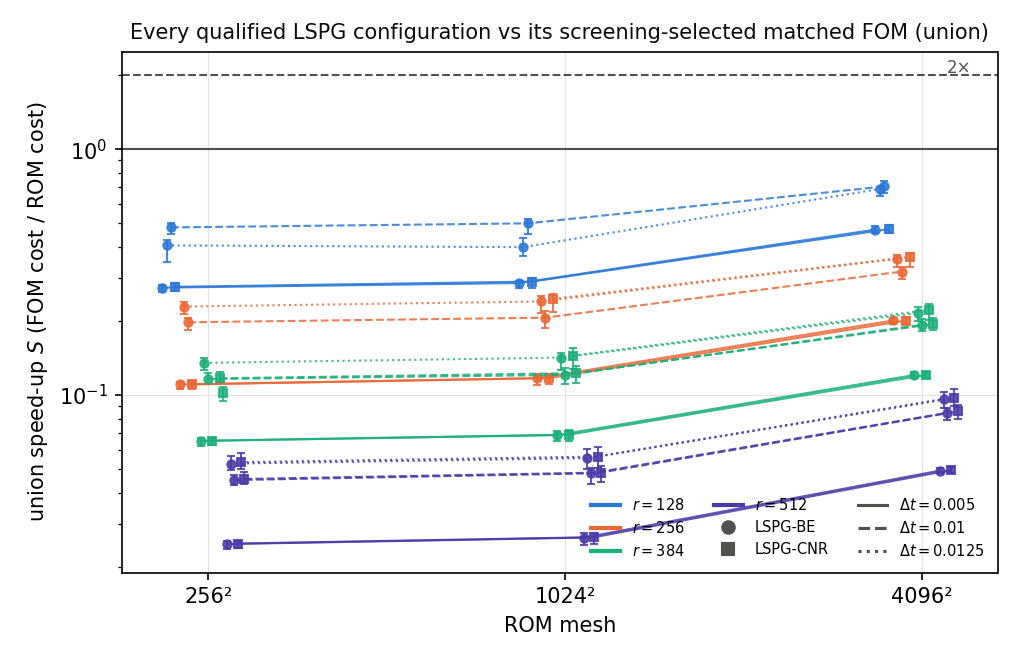
\includegraphics[width=0.48\linewidth]{figs/f2_speedup_vs_mesh.png}\hfill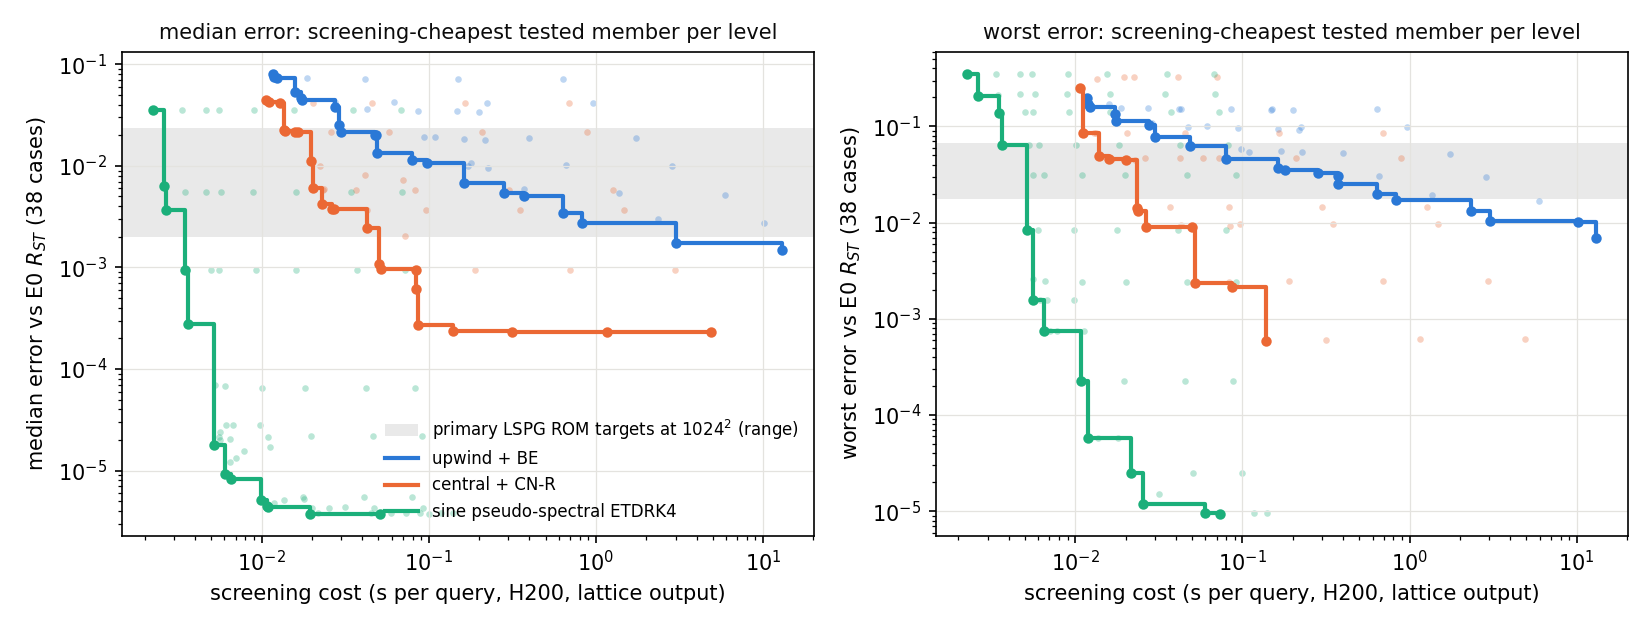
\includegraphics[width=0.48\linewidth]{figs/f2_fom_pareto.png}\end{center}

\subsection*{Consequence and corrections}
With K2 firing in both 2D and 3D, the plan's written consequence applies: no ``substantially faster than the best full solver'' claim; the paper leads with mesh-independent cost (and memory), and reports speed-ups against named comparators with their scope. \retracted{The combined lane's H5 speed-up (13.6$\times$ selected scheme, 17.7$\times$ best arm) holds only within its scope --- a same-mesh upwind FOM matched on worst error --- and does not survive the expanded ladder. Spectral at the ROM's own resolution and the governing plan's other solver families (upwind+CN-R, Newton--GMRES, IMEX-CG) were not run.}
